%----------------------------------------------------------------------------------------
% PACKAGES AND OTHER DOCUMENT CONFIGURATIONS
% WARNING: Don't mess with any of the following unless you know what you are doing.
%----------------------------------------------------------------------------------------
\documentclass[english,12pt,a4paper,openany]{book}
\usepackage{datetime}
\usepackage{tabularx}
\usepackage{makecell}
\usepackage{eurosym}
\usepackage{pbox}
\usepackage[utf8]{inputenc}
\usepackage[T1]{fontenc}
\usepackage[english]{babel}
\usepackage{amsmath}
\usepackage{amsfonts}
\usepackage{fancyhdr}
\usepackage{amssymb}
\usepackage[dvipsnames]{xcolor}
\usepackage{mdframed}
\usepackage{multirow}
\usepackage{multicol} 
\usepackage{tikz}
\usepackage{graphicx}
\usepackage[absolute]{textpos} 
\usepackage{colortbl}
\usepackage{array}
\usepackage{geometry}
\usepackage{hyperref}
\pagestyle{fancy}
\renewcommand\headrulewidth{1pt}
\usepackage{float}

%------------------------------------------------------------------------------------------------------
%	The following are the RGB values for the official ATU colours.
%------------------------------------------------------------------------------------------------------	
\definecolor{ATUGreen}{RGB}{0, 91, 94}
\definecolor{ATULightGreen}{RGB}{172, 245, 189}
\definecolor{ATUNavy}{RGB}{0, 26, 121}
\definecolor{ATUOrange}{RGB}{255, 121, 30}
\definecolor{ATUPurple}{RGB}{77, 8, 87}
\definecolor{ATUSand}{RGB}{255, 232, 212}
\definecolor{ATUTeal}{RGB}{123, 185, 203}
\definecolor{ATUWarmGrey}{RGB}{200, 190, 191}
\definecolor{ATUYellow}{RGB}{248, 255, 142}



%------------------------------------------------------------------------------------------------------
%	******* CHANGE THE FOLLOWING VARIABLES
%------------------------------------------------------------------------------------------------------	

\newcommand{\reportauthor}{David Amankwah} % Change to your name
\newcommand{\projecttitle}{ConnectSphere}
\newcommand{\reporttype}{Minor Dissertation} %Report  type (Project Plan / Final Report)
\newdateformat{monthyeardate}{\monthname[\THEMONTH], \THEYEAR}





%------------------------------------------------------------------------------------------------------	
% WARNING: Don't mess with any of the following unless you know what you are doing.
%------------------------------------------------------------------------------------------------------	
\pagestyle{fancy}
\fancyhf{}
\fancyhead[R]{\textcolor{ATUGreen}{\reportauthor}}
\fancyhead[L]{\textcolor{ATUGreen}{\projecttitle}}
\fancyfoot[L]{\textcolor{ATUGreen}{Atlantic Technological University (ATU), Galway.}}
\fancyfoot[R]{\thepage}

\begin{document}
\begin{titlepage}

\newgeometry{left=6cm,bottom=2cm, top=1cm, right=1cm}

\tikz[remember picture,overlay] \node[opacity=1,inner sep=0pt] at (2.2mm,-165mm){
\includegraphics{images/leftbar.png}}; % Fond changeable 

\fontfamily{fvs}\fontseries{m}\selectfont
\color{white}

\begin{picture}(0,0)
\put(-110,-743){\rotatebox{90}{\Huge{B.Sc. (Hons) in Software Development}}}
\end{picture}
 
\vspace{-10mm} 

\flushright 
\includegraphics[width=100mm]{images/atu-logo-green.png} 

\flushright
\vspace{10mm}
\textcolor{ATUGreen}{
\fontfamily{cmss}\fontseries{m}\fontsize{22}{26}\selectfont
\projecttitle
}
\normalsize
\color{black}

\vspace{1.5cm}
\normalsize
\textbf{By \\ \textcolor{ATUGreen}{\reportauthor}}\\ 
\vspace{15mm}
{\scshape \today} \\[0.3\baselineskip]
\vspace{75mm}
\Large {\textcolor{ATUGreen}{\textbf{{\reporttype}}}} \\
\bigskip
\normalsize
\textbf{Department of Computer Science \& Applied Physics,\\School of Science \& Computing,\\Atlantic Technological University (ATU), Galway.}\\
\end{titlepage}
\newpage
\tableofcontents
\listoffigures
\listoftables
\pagenumbering{arabic} 

%----------------------------------------------------------------------------------------
%	   ******* CHANGE the Chapters if necessary. Each chapter is encapsulated inside 
%                 its own file. The chapters below are based on the guidelines 
%                 given in the lecture.
%----------------------------------------------------------------------------------------
\chapter{Introduction}

Social media is ubiquitous in our daily lives, providing users with a platform to connect online, share content, and build communities \cite{ishaq2023design}. When interacting with other people's posts on the internet, users may experience a wide range of emotions, including frustration, excitement, joy, and dejection \cite{tanna2020sentiment}. As the number of people using social media has grown over time, social media applications have become a very common aspect of using the internet \cite{aichner2021twenty}. When users share online content to educate other users about global events, social media applications can be used very effectively \cite{yu2022social}. Social media applications also assist businesses in expanding by offering online services to meet the needs of their clients \cite{go2016but}.

\section{Background}
Over time, people's methods of exchanging information and content have changed, and social media platforms like Facebook and YouTube have had a lasting impact on society \cite{komito2011social}. Social media have been promoted as a means of fostering human connections and enabling communication. Social media gives users the ability to search for other profiles, have a public profile, and a list of other users they are connected to \cite{leist2013social}. People of all ages can now interact with friends, family, the educational system, and society through social media \cite{wilkinson2015social}. A billion users share content and information online via social media platforms like Facebook, YouTube, Twitter, and Instagram \cite{wilkinson2015social}.

Modern web applications are responsive and fast. This development for web apps has allowed users to have a smooth experience. Users expect to have fun while surfing the web, and this is what makes social media comfortable for so many users. Users can connect with important people and things that matter when a website offers them quality features that make them feel good, and that's exactly what the Internet has become. When the internet began, changes were made to web technologies such as HTML, CSS, React, Express, Node and JavaScript in order to create the best possible website for users \cite{aryal2020mern}.

\section{Motivation}
This project aims to build a social media platform that securely creates user engagement through features such as posts, likes and comments. Developing numerous advanced features to design an engaging and easy to use social media platform. User engagement is about how someone feels about the content that is presented on the page, which can show strong positive engagement \cite{shahbaznezhad2021role}. A successful social media platform must have diverse content and offer the opportunity to spread content to a very large audience of site visitors \cite{khan2017social}. A social media platform should focus on information consumption at a deeper level by looking at engagement in the form of likes, dislikes, comments, shares, uploads and views in a way or another \cite{khan2017social}.

The social media application uses the web technologies such as React, MongoDB, Express and Node to create a platform where users can stay active while interacting with the social platform. Web technologies are growing rapidly, and MERN full stack is popular for handling the front-end and back-end with the help of JavaScript support on the client side and server side \cite{aryal2020mern}. 

\section{Objectives}
\begin{enumerate}
  \item To enhance user engagement through the implementations of features such as posts, likes, dislikes ,images, and user interactions.
  \item Create a secure user authentication using token-based methods user login and registrations.
  \item Dynamic content support for updating and deleting user-generated posts.  
  \item Allow users to follow and unfollow other users on the platform. A recommendation system to help users get started on following a user.
   \item A Search functionality for users to search others by username with responsive search results.
   \item A user profiles for showing important details and follower counts.
   \item Learn and develop best practices using various
   technologies in the MERN stack. 
   \item Gain project building skills.
\end{enumerate}

\section{Problem Domain}
Developing a social media platform is all about managing with the expectation of users of this generation where the influence of the Internet's is very powerful. The integral parts that social media should provide are the sharing different forms of information for the users to interact and engage, with likes and comments \cite{go2016but}. A community is created for users to enjoy. Companies are very careful to select and connect features of social media applications, such as expression and sharing, to create a growing community \cite{go2016but}. In today's world, social media is an important modern form of communication, connecting so many people and creating a different ways of interaction, including sharing opinions, images and messages. 

Social media is accessible so that users can use it for free with complete privacy protection, social media has preferences that allow users to make updates according to their preferences, and social media has a reach that allows websites to gain a global audience \cite{agarwal2010information}. There are challenges and opportunities to overcome when creating a user-oriented social media platform that offers different preferences and features. The most common challenges are securing user privacy, implementing user authentication, handling dynamic content, and making the environment engaging and interactive for the user to enjoy. 

\section{Project Overview}
This dissertation displays the development of a dynamic and user-oriented social media platform called ConnectSphere. The aim is to build an engaging digital space to enhance user interaction. The project aims to create a pleasant social media experience, ensuring seamless and responsive platform for users to enjoy, share, connect and communicate.

The MERN stack is used for the project objectives, combining both the front-end and back-end technologies. The front-end is built using React, a JavaScript library for creating user interfaces, and Material-UI guarantees responsive styling of components. The back-end is built using Node.js for the server-side development, ensuring stability and efficiency. Express.js, a framework for Node, which simplifies server side development code. MongoDB is used as a database and provides a way to store and retrieve data. JSON web token provides a secure user authentication, improving the platform's security. Security is a key aspect for a social media platform. Redux toolkit is used for state management. This social media platform focuses on providing various features to enhance the social media experience. Users are encouraged to interact, fostering a dynamic and responsive community. The technologies used in this project, helps creates a social media platform, providing users with a secure and engaging online community.
\chapter{Methodology}
The goal of the project was to build a social media platform that would allow users to enjoy content and interact in a meaningful ways. Users can share posts from other users. The MERN stack of MongoDB, Express.js, React.js and Node.js, is used to develop the social media platform. The growing popularity of social media platforms focused on user engagement is the main reason to start the social media project. ConnectSphere was created using an Agile software development methodology. The Agile approach allows for an iterative development cycle. The objective was to create a community where users to could communicate through various features such as posts, comments and messages. 

The project involved trying to create a social media application from scratch and developing project creation skills. Learn about useful approaches for a MERN stack application using various technologies. While coding the project, react router, formik and yup, JSON web token, dropzone, redux toolkit, and multer were all learned for the front-end and back-end implementation. The back-end was initially implemented to configure middle-ware, controllers, models, routes and database connections. Once the back-end was fully implemented, the front-end configures widgets, components and pages. The front-end encountered some difficulties during the design of the project. The back-end was less difficult but there were few a difficult encounters. This sections provides an overview of the methodologies employed throughout the development and research phases of the project. The software development methodology and the technologies implemented played an integral part of the project.

\section{ Software Development Methodology} 
The software development methodology used for this project is an agile approach, mainly the Scrum framework. The Scrum implementation is used to the deliver the social media platform and to understand what can be the most effective in terms of delivering the social media project \cite{garzaniti2019effectiveness}. Agile methodologies focus on iterative and incremental development, allowing flexibility and responsiveness to any change request. The project had to meet many requirements to further develop the social media application. Many features have been taken into consideration in order to enhance the project and make it more attractive for users. The agile approach made the project more organized and reduced the risk of the loss of control. Scrum, with its iterative sprints and regular feedback loops, demonstrates the importance of managing the dynamic aspects of developing a social media platform. The social media platform had features to achieve during the coding. New requirements had to be adapted to ensure smooth during the development. The agile approach has proven to be a reliable step towards achieving certain functions. Project development involved the use of sprints to control and organize the development. During the sprints, the tasks selected for the project were processed. All issues related to the progression of the development have been studied. The development was reviewed to ensure the project was on track and functioning properly. The goal of the sprint was to deliver a social media application that allowed for users to communicate. Regular sprint reviews allowed the project to continuously improving and adapt to changing requirement and challenges each week.

\subsection{Agile Methodology}
Agile Methodology is an effective software development method. The iterative and incremental approach to software development focused on the flexibility and users need. It enabled dynamic planning and quick delivery of functional increments. Incremental requirements refine the design, coding, and testing at all phases of production activity \cite{kumar2012impact}. The goal of Agile Methodology is to develop high quality software in a short time, be self organizing, focus on user needs, require fewer documents and reduce the time to market \cite{kumar2012impact}. The requirements may change as the tasks are divided into multiple iterations to create a release plan that advance the project through the iteration phase \cite{altameem2015impact}. The product backlog contains all the bug fixes, requirements, features, and non-functional requirements that an effective software must address \cite{altameem2015impact}.

Adaptability is very beneficial to project management because agile embraces changes in requirements so that to allow a developer can respond to changing project requirements. Agile methodology has emerged to serve as a replacement for traditional methods of software development methods that were very limited and predictable \cite{altameem2015impact}. Agile methodology ensures a developer can handle various aspect of development, including coding, testing and deployment. Agile ensures that the product meets user expectations. The project focuses on the needs of user of a social media platform. Agile methodology promotes trust, improves the trust between the developers and users and shows that it is beneficial for a project \cite{altameem2015impact}.

\subsection{Scrum}
Scrum is a very popular framework within the agile methodology. It provides a structured and flexible way to develop software. It contains many important elements that help developers improve their ability to create quality software application. Scrum contains a set of rules and responsibilities that never change in order to help the developer ensure that the quality, stability, time, cost and control of the product are in good condition \cite{darwish2016requirements}. Scrum ensures that a project is delivered in the best possible way because it helps developers solve complex problems \cite{darwish2016requirements}. User expectations from the project take priority when a project is delivered for publication. A product backlog, sprints, and increments manage project tasks and bugs to create a project release. With the help of the Scrum framework, project work can be planned well. It provides a sprint retrospective to reflect on the sprint and look for opportunities for improvement. Scrum promotes transparency, adaptability and continuous improvement. 

\section{ Technologies Used} 
The technologies used for the social media platform help shape the blueprint to create a successful application. The technologies used for the project are diverse and include a range of tools that adapt to the requirement and objectives of the project.

\subsection{Frontend Technologies}
\subsubsection{React.Js}
The frontend of the social media platform is developed using the React library. React is really focused on project delivery thanks to its modular and reusable UI components, made possible by a component-based architecture. React has provided a responsive and interactive user interface. React ensured a robust and versatile social media platform. The use of React is an important aspect of the project's attractive application features. React is a reliable programming technology if you need to develop a dynamic user experience for a social media application. The functions and features of the project were all developed using the components used to develop them. React made it possible to seamlessly implement design the social media application design with these features.

\subsubsection{Material-UI}
The style and visuals representation of the project was handled using the reliable technology called Material-UI. Material-UI ensured a consistent and aesthetically pleasing design. The React UI framework provides a set of predefined components that follow the principles of Material-UI. The use of Material-UI was very consistent across use the rest of the social media platform.

\subsubsection{Dropzone}
Uploading images from the project was handled very well with Dropzone. React Dropzone is integrated for image upload usage. Dropzone is a way for users to upload directly from their local file system to a  designated area on the web page. Dropzone is useful for having images on the social media platform. 

\subsubsection{Formik and Yup}
Formik and Yup are very popular libraries in React and they are often used together for form management and validation. The purpose of Formik is to help manage form status and manage form submissions. Formik offered a dynamic form for user login and registration. The purpose of Yup is for value parsing and validation. Yup works with Formik for defining validation rules for form fields.

\subsubsection{React Router}
React Router is a useful library for handling the navigation in the social media application. This allowed users to switch between different parts of the application without having to reload the entire page.

\subsubsection{Redux}
The project included a way to manage state called Redux. State management in the frontend managed by Redux, a predictable state container for the social media application. Redux has been implemented for efficient state management in the frontend. Redux ensured the stability and maintainability of the frontend. It has provided access to the efficiency of state management to manage complex interactions within the social media application.

Redux state management is used to ensure that the web application is scalable and maintainable, especially when dealing with difficult state interactions. Redux aims to predictably handle state mutation without losing the performance benefits of asynchronous and making the application is easier to test \cite{bugl2017learning}. Redux was very efficient in controlling and organizing the different states in the social media platform. It is effective in ensuring that the application meets the projects objectives. The main concepts of Redux include Store, Action, Reducer and Dispatch. The Store is a JavaScript object that stores state of the application because it is a container containing the state tree. The action describes the application state change. Reducers specify changes in application state changes in response to actions. Dispatch is a method that is used to dispatch actions that trigger the reducer to execute for the new state.

\subsection{Backend Technologies}
\subsubsection{Node.Js}
The backend server of the social media platform is built using the Node.js, known for its scalability. Node.js made it possible to handle a large number of simultaneous connections, which is crucial for the social media platform. Node.js enabled robust server-side development. Node.js is ideal for building scalable and high performance web applications, and  is often used with Express.js to develop web servers and applications. 

\subsubsection{Express.Js}
Express.js is a flexible Node.js web application framework that supports developers in building robust web servers. Express.js makes it easier for developers to create web applications and APIs by providing an organized structure. Express can be used to create APIs with the endpoints that handle various HTTP methods, making it a very popular tool for creating backends. Express has an efficient routing system that allows developers to define routes based on URL and HTTP methods. This made it easier to create users authentication and posts on the social media application. Express.js has also taken an approach with its middleware system that allows developers to extend the functionality of the web applications. You can add Middleware function to perform various tasks such as error handling and authentication.

\subsubsection{Bcrypt}
Bcrypt is a password hashing function that is used to securely store passwords in a database. It is designed to be adaptable, ensuring a strong password hashing option. Bcrypt is the best choice if you are implementing a password storage instead of trying to create a custom one. On the social media platform, bcrypt is used for secure hashing of passwords during the user registration and authentication during the user login. Bcrypt is useful for protecting user passwords in the database by storing them in a hash format with additional features such as salting.

\subsubsection{JSON Web Token}
JSON Web Token (JWT) is used in the project for security purposes. The
social media platform must to be secure, and JWT is used to add security to the user's information. JWT is used for user authentication, posts and secure user data. Its very important to handle the JWT securely and store them properly. A middleware function is implemented in the project which checks if a JWT is present in the header of an incoming request. If a valid token is found, it is validated using the JSON web token library. If the verification succeeds, the decoded payload is attached to the user request object. The middleware is designed to be inserted into the middleware chain before routes that require authentication. The middleware ensures that only requests with valid JWT can proceed to the protected routes, and is added to the decoded user information for further processing.

\subsubsection{mongoose}
Mongoose is an object data modeling library for Node.js and MongoDB. It provides a simple schema-based solution for modeling web application data and connecting to MongoDB. Mongoose makes it easy to communicate with MongoDB by providing a structured way to design schemas and perform CRUD (create, read, update and delete) functions. 

\subsection{Database}
\subsubsection{MongoDB}
The database used for the social media platform was the MongoDB. MongoDB is a well-known open source NoSQL database management system. MongoDB was chosen for this project because it offers flexibility, scalability and good performance. MongoDB is a suitable choice for building a social media platform. MongoDB is widely used in web applications and other scenarios where a dynamic and scalable database solution is required. MongoDB was used to store user data, posts, and other relevant information in a format that fits well with the flexibility of a social media platform. Data could be retrieved from the MongoDB to display on the platform.

\subsection{Project Management}
\subsubsection{Jira}
Jira is a very popular project management tool that is used to help developers to plan, track, and manage their work. Jira is widely used in software development and helps manage the social media platform creation process. Jira allows a developer to create and track issues, tasks, and other work items. It supports project planning and task assignment for the social media platform.
\chapter{Technology Review}
This chapter discusses the technological landscape of social media platforms and the specific technologies used in the ConnectSphere project. It was necessary to research the design need of the social media platform for the user experience. This review provides a foundation for the understanding the choices made in the development process and how they connect the goals of social media applications. Frontend and backend were important aspects to develop features for the applications. Jira was the project management tool to help manage the project and MongoDB for data storage. Other tools used allowed the developer to build the social media platform in order to achieve the set goals.

\section{Social Media}
Since the creation of social networks in 1997, the main purpose of social media application has been to facilitate people in terms of social connectivity \cite{shabbir2016impact}. The social media platforms provides people with natural ways to help them enjoy their lives and stay connected, as well providing different types of information, but it is 
 also a place where users can create media and content \cite{shabbir2016impact}. These aspects for are taken into consideration in the development of the project to promote users involvement, and create a seamless experience environment. The goal of the project is to create features such as posts, likes, images, comments and user interactions in order to develop a compelling user experience that encourages active participation. The motivation for any social media platform like Facebook, Twitter, and Instagram is to connect with people who share to similar interests \cite{shabbir2016impact}. Social media applications are all about constant communication to create a community for users, and maintaining that communication is a crucial part \cite{jain2014application}. 

 \section{React.js}
 React is a powerful frontend technology that is used to develop web applications \cite{rawat2020reactjs}. The project used the React framework to develop the frontend of the social media application using JavaScript. React is a reliable technology with the numerous advantages that make it easier to develop an attractive web application. React offers incredible performance, especially with the JSX, where JavaScript and XML works very well together \cite{rawat2020reactjs}. React is a popular framework that offers many other features to design the best user interface for a social media platform. React offers dynamic features like routing where the web applications are rendered on the machine \cite{rawat2020reactjs}. React provides the Redux library and this feature brings many enhancements within the components to render them when needed \cite{rawat2020reactjs}. React Redux also produces a container function as a wrapper component to determine with the way towards collaboration path with the store \cite{rawat2020reactjs}.

 React can be integrated with the Node.js backend using many APIs such as the RESTful API \cite{ishaq2023design}. React allows developers to efficiently create reusable UI components and manage the state of web applications \cite{ishaq2023design}. The API used in the project could 
 able to work smoothly with the backend to retrieve and store information about users and their content from the database. React provides hooks that allow developers to write class-based components by handling state management from functional components \cite{aryal2020mern}. The main purpose of hooks is to solve problems when writing functional components that have access to state, context and life-cycle methods \cite{aryal2020mern}.

\section{Node.js and Express.js}
In Node.js, developers create business logic in the backend of a web application \cite{shah2017node}. Node.js is a popular open source web server that allows developers to create dynamic web applications \cite{aryal2020mern}. Node.js can handle many requests by running a single thread \cite{shah2017node}. Node.js requires developers to know only a single language, such as JavaScript, which is an advantage it has over other backend frameworks \cite{shah2017node}. Node.js is highly  performant, and it uses JavaScript because JavaScript provides first-class functions and closures \cite{syed2014beginning}. Node.js allows developers to create models that are abstractions of the data in the MongoDB \cite{ishaq2023design}. 

Node.js is known for creating a single page application and adding features to it \cite{shah2017node}. Node.js is a bit difficult for developers to learn, but the learning curve is not that steep \cite{shah2017node}. Setting up event-driven functionality of feature is also a challenge for some developers, but Node.js is has the advantage of easily configuring your hardware or server in an organized way \cite{shah2017node}. Before Node.js it was difficult to learn languages to build on the server and client side, now developers can build powerful and fast applications for a MERN stack with Node.js \cite{shah2017node}.
Express.js is a minimal and dynamic Node.js web application framework that provides developers with functionality to build various web applications in a MERN stack \cite{ishaq2023design}. Express.js is clear and easy for developers to use because it provides an API for routes and handling HTTP request and middleware \cite{ishaq2023design}. Express.js provides middleware features with requests, response and a middleware function. The middleware breaks the request handler into multiple steps and run code to make changes to the request and response objects \cite{peters2017building}. Express.js has built-in functionality to handle incoming HTTP requests with a route associated with the request handler with the primary purpose of performing CRUD operations \cite{peters2017building}. Express has a helper function that sends static files, such as HTML and CSS files, to client side
\cite{peters2017building}. Both Express.js and Node.js are powerful server-side technologies that offer many advantages. There were few problems to with its operation, but there weren't many problems.

\section{MongoDB}
MongoDB is a NoSQL database that offers developers a scalable and flexible way to manage data \cite{ishaq2023design}. MongoDB provides persistence for app data and designed is scalability and developers \cite{aggarwal2018comparative}. This is a positive for developers building an application that needs a maintainable database. MongoDB solves the gap issues between key-value pair stores, which are quick and scalable databases \cite{aggarwal2018comparative}. MongoDB allows you to use of internal memory to store working sets for faster access to data \cite{aggarwal2018comparative}. Other benefits offered by MongoDB include clear object structure, simple join, tuning, schema-free, and deep quires \cite{aggarwal2018comparative}. These are some of the reasons why MongoDB is popular when creating a project to store data in database. There are some drawbacks to using MongoDB. The disadvantages of MongoDB are the gigantic data size, less flexibility in query execution and lack of
transactional support \cite{aggarwal2018comparative}. MongoDB is a document-oriented database with no joins or transactions to make writing queries easier \cite{zhao2013modeling}.

MongoDB supports indexing, allowing you to index to any attributes in the database, and secondary indexes are also available \cite{zhao2013modeling}. Replication in MongoDB has support for master and slave replication, which provides redundancy, backup and automatic fail over \cite{zhao2013modeling}. Load balancing in MongoDB scales horizontally by using partitioning to distribute only a single logical database system across a group of machines \cite{zhao2013modeling}. MongoDB has the ability to be used as a file system that can store any file using the GridFS functionality \cite{zhao2013modeling}. MapReduce is supported by MongoDB and allows users to retrieve results using the SQL group-by clause \cite{zhao2013modeling}. All these additional features supported by MongoDB show how reliable it is for developers to use for when managing their database while building an application.

\section{JSON Web Token}
It is very important for user authentication and access management in web applications because it is necessary for network security \cite{ahmed2019authentication}. JSON Web Token (JWT) is a JSON object that provides a secure approach to representing a set of information between two parties \cite{ahmed2019authentication}. JWT represents the claims format for restricting the scope of an environment such as HTTP authorization headers and URI request parameters \cite{haekal2016token}. The claim is encode by JWT to be sent as a JSON object that is used as a payload, so the claims can to be a digitally signed message authentication code \cite{haekal2016token}. The server side uses JWT for queries until users log out of the application \cite{ahmed2019authentication}. One of the main functions of JWT is to enable state transition for communication, while a client cannot modify the information contained in the token \cite{ahmed2019authentication}. The JWT header has information about the JWT signature to be computed, the JWT payload has the data stored in the JWT, which could be an id or email, and the JWT signature has the signature of the header and payload \cite{ahmed2019authentication}.

Clients sends a username and password authentication request that is verified by an authentication service that creates a JWT based on the retrieved user authorization data \cite{ahmed2019authentication}. The token is used by the client with the request to a secure resource on the server, and the server receives the request to extract the user's authentication data from the JWT to send a response based on a valid or invalid token \cite{ahmed2019authentication}. implementing of token-based authentication using JWT on RESTful web services as an alternative to replacing server-based authentication \cite{haekal2016token}. JWT is considered a scalable solution providing performance benefits for user access control in large scale systems and there is a need to provide a general solution for all types of applications \cite{ahmed2019authentication}. JSON Web Token provides the security needed to build a web application.

\section{Socket.IO}
Socket.IO is similar to a web socket in that it provides the ability for real-time communication between the client and the server \cite{gelens2014gevent}. The idea of Socket is that it is a virtual socket, which abstracts from the fact that the transport does long-polling, and provides other functions similar to web sockets for all \cite{gelens2014gevent}. When building a unique web application, Socket.IO provides developers with reliable technology to create features like notifications and a live chat. Socket provides two way communication that connecting two programs running over the network \cite{joby2016socket}. The basic steps to create the socket are to open the socket, wait for the client, establish communication with the I/ O flow, perform communication and then finally close the socket \cite{joby2016socket}. This allows for real-time communication between the server and the client to really be efficient. With Socket.IO, a chat function can be managed efficiently,
enabling a flexible and modular communication model. Socket.Io makes it easy to implement a notification functionality with real-time communication between client and server to produce instant updates. Socket.IO is a powerful tool for creating a real-time communication web application with fast and efficient communication between server and client. 

\section{Jira}
To create an efficient applications, project development necessitates careful planning based on objectives and goals. Developer's work heavily relies on project management. Jira is a popular and useful tool for project management. Atlassian developed Jira as an issues tracking system in 2002 \cite{fisher2013utilizing}. Jira provides developers with a variety of tools for local customization to meet project requirements,
including issue types, workflows, and user stories \cite{fisher2013utilizing}. When an issues is submitted, a member of the project team automatically notified and assigned to a specific task of the project \cite{fisher2013utilizing}. Assigning tasks to developers for specific tasks in the project allows for a clear focus on achieving the goals of application development. Review teams conduct design and code reviews to assess the complexity of software effort, aiming to ensure software quality assurance \cite{fisher2013utilizing}. Jira ensures that developers focus on the coding of the project in order to stay organized with the application requirements. Jira lacks the capability to regulate the modifications made to the specific fields in a Jira issue, allowing only authorized users to make changes if the specific fields are available on the entry screen \cite{fisher2013utilizing}.

Jira has a custom Scrum board and dynamic Kanban board, which seamlessly integrate with popular environments, are essential components of its functionality \cite{ozkan2019agile}. In addition, Jira provides bug tracking, flow diagrams, custom developer tools, and issue and reporting capabilities \cite{ozkan2019agile}. Jira has established itself as a trusted tool that is widely used by developers and large organizations \cite{ozkan2019agile}.  

\section{Render}
The ConnectSphere social media application is scheduled for deployment once the completing the design and functionality testing are finalized. Render is the tool utilized to deploy the web application. Render is a cloud application that enables the deployment of MERN stack applications, emphasizing the important of having a reliable deployment mechanism. Cloud applications offer a robust computing platform to build a application on top of the platform \cite{fylaktopoulos2016overview}. The application developer is solely responsible for developing the application, while the cloud application take care of maintaining the platform \cite{fylaktopoulos2016overview}. Render provides a variety of services, including databases, Secure Socket Layer certificates and domains. Render allows developers to easily deploy and scale their web applications across a large infrastructure, without having to worry about the server management and scaling \cite{ssemakula2023low}. GitHub, GitLab and Docker are popular development tools that integrate with Render to make it easy to deploy an application and manage the infrastructure \cite{ssemakula2023low}.
\chapter{System Design}
This chapter will describe the system design of ConnectSphere project, including the frontend and backend architecture, as well as how different components interact to deliver the desired functionality. The frontend of ConnectSphere is developed using React.js, a JavaScript library for building the user interface. The backend of ConnectSphere is built using Node.js and Express.js to provide a reliable server-side environment. This section will present the overview of the frontend and backend architectures. MongoDB was also used to store and retrieve data from the web application.

\section{System Interaction}
The web application works when the frontend interacts with the backend through API requests and responses. When a user creates
or updates a post, the frontend can send an HTTP request to the API endpoint on the backend. The request is processed by the backend. The backend performs the necessary CRUD operations and returns the desired results. The interactions between the  frontend and backend are seamless, allowing for real-time updates and data synchronization throughout the application.

The frontend represents the user interface of the web application, created using technologies such as React and Material-UI. it send HTTP request the backend API to retrieve or manipulate the data. The backend server of ConnectSphere, implemented using Node.js and Express.js. It receives HTTP request from the frontend, performs the necessary operations and return the appropriate response. ConnectSphere uses MongoDB for its flexibility and scalability. MongoDB is where the application's data is stored. The backend interacts with MongoDB to perform the CRUD operations on the data. HTTP requests are made by the frontend to communicate with the backend API. This includes requests to retrieve user data, publish new content, or update user information. After processing the requests and interacting with the database, the backend API return responses with data and status code. The frontend uses this data to update the user interface accordingly. The database operation is performed by the backend API on the database in response to incoming  HTTP requests. Figure 4.1 provides an illustration of the UML diagram. The UML diagram provides an overview of how the various components of ConnectSphere interact with each other to facilitate the flow of data and operation within the application.

\begin{figure}[h!]
    \centering
    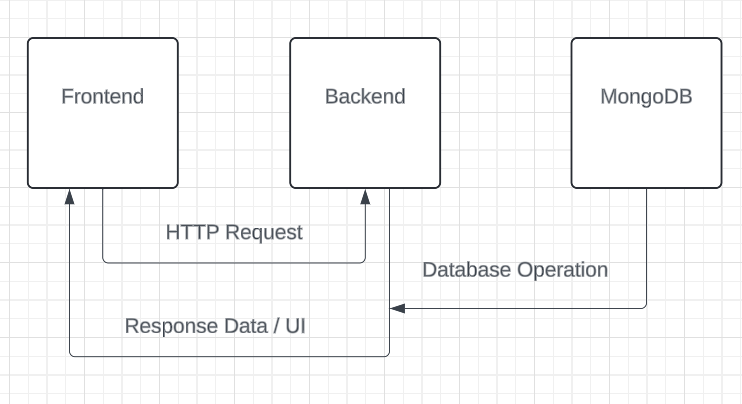
\includegraphics[width=0.7\textwidth]{images/uml.PNG}
    \caption{UML Design}
    \label{fig:uml-design}
\end{figure}



\section{Frontend Architecture}
\subsection{Component-based Structure}
The ConnectSphere uses a component-based structure, with different UI elements are encapsulated within reusable components. This approach enabled the coding process to be flexible and dynamic. Components were combined to build complex user interfaces while keeping the code organized. Each component in the web application serves a specific purpose throughout the application. When creating a post with which users can interact, a component was created to handle all of the post's operations. Another component was designed to display posts, either for the entire application or for a specific user. There is also a component to edit and update a user's post. This allowed the post to be displayed on the home page, where users could interact. Components are imported into other components to extend the application's functionality. The React component-based architecture promotes code reuse effectively. Figure 4.2 depicts the code rendering EditsPostForm component.

\begin{figure}[h!]
    \centering
    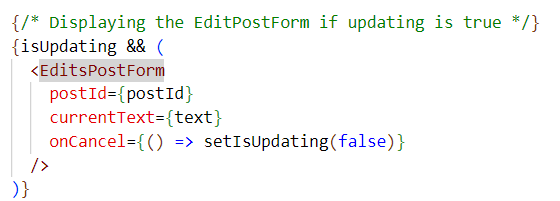
\includegraphics[width=0.7\textwidth]{images/component.PNG}
    \caption{Code snippet from PostWidget.jsx to show EditsPostForm component}
    \label{fig:reusable-component}
\end{figure}

\subsection{Material UI Integration}
Material-UI is a popular React UI framework. Material-UI is integrated into the web application to ensure consistent styling and responsiveness across the social media platform. Material-UI provided numerous pre-built components and styles to help the design of the web application. The design of a social media platform is critical for the project. Material-Ui enabled the application to include important icons for chats, searches and notifications when developing a web application. Material-UI has made ConnectSphere to feel more natural by improving the user interface throughout the application. The social media application can be displayed effectively and simply thanks to the Material-UI tools.

Overall, Material-UI enabled ConnectSphere development to create a visually engaging, responsive, and accessible user interface while maintaining consistency throughout the development process.

\subsection{Redux State Management}
Redux is used to manage the application state, particularly for handling complex state interactions such as user profiles, user authentication, post management and following management. Using Redux state management, the application has a predictable state. The Redux toolkit is used to create slices of state along with their associated reducers. Reducers are defined in each slice that specify how the state should be updated in response to dispatch actions. These slices allow the application to update a user and token in the state when a user sign in or signs out. Specific actions are exported from the slices using destructing, allowing certain parts of the application to import and dispatch these actions. State updating is centralized and consistent across the entire web application.

Actions defined in the slice updates the state immutably. The Redux toolkit handles immutability behind the scenes, allowing for instant state updates without having to worry about modifying the original state object. Redux hooks such as useSelector are used in web application components to access certain parts of states and dispatch actions using useDispatch.

\subsection{API Integration}
The frontend interacts with the backend API endpoints to fetch and update. This allows for communication between the frontend and backend components. Functions are created to handle data fetching operations from the backend API and are typically called when the components are deployed or when certain conditions are met. RESTful API interaction is demonstrated by fetching and handling asynchronous operations using async and wait. Redux actions are dispatched to update the state of the web application with the retrieved data so that it is available to other components. The architecture is designed to follow the best practices for separation of concerns, ensuring that data retrieval logic is isolated from user interface components. Figure 4.3 shows a code snippet for handling comment submissions in a web application.
\begin{figure}[h!]
    \centering
    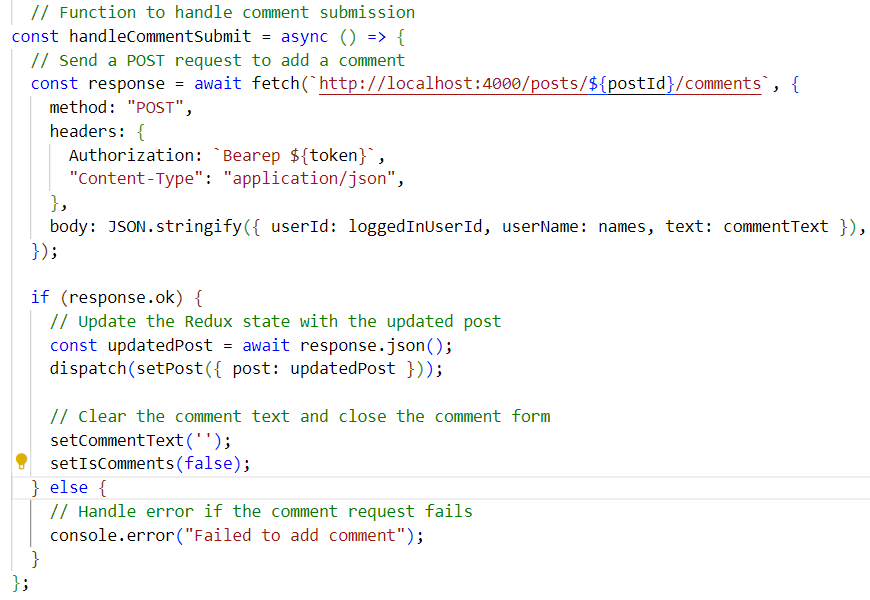
\includegraphics[width=0.9\textwidth]{images/function.PNG}
    \caption{Code snippet from PostWidget.jsx to handle comments}
    \label{fig:comment-function}
\end{figure}

The GET request is used to retrieve the all data from the backend API. The POST, PATCH, and DELETE requests are used in functions to perform various actions, such as liking a post, deleting a post, and adding a reply to a comment. Bearer token is included for authentication, ensuring that only authorized users can perform certain actions like liking post or deleting post. If the response is positive, the Redux state is updated with the updated actions. Error handling is implemented to detect and log any errors that may occur with API requests. Each API interaction is encapsulated in its own function, promoting modularity and code reusability. Socket.IO is used for real-time communication to alert users of certain actions. This improves the user experience by providing instant updates without the need to manually refresh the page. 


\section{Backend Architecture}
\subsection{RESTful API Design}
ConnectSphere follows a RESTful API design pattern where different routes correspond to certain CRUD operations. This allows the application to have a clear and predictable API structure. Making it easier to develop and maintain the backend.
Following RESTful principles for the backend API design ensures a good approach to building scalable and maintainable APIs. Routes are organized around resources such as users and posts, which aligns with RESTful principles. HTTP methods are used to retrieve data, partial updates, delete resources  and create new resources. Parameters are used in the routes to identify certain resources or perform on them.

Error handling is implemented using try-catch blocks in the controller functions to catch errors and send the appropriate HTTP status code along with the error message. This allows the coding process to go smoothly. The error messages pointed to application development issues. The status code indicated whether the error came from the frontend or backend. A middleware function such as 'checkToken' is used to handle the authentication, which is a common practice in RESTful API to ensure security. Security is a crucial aspect of ConnectSphere because it is a social media platform and social networks prioritize security. There is dedicated user search endpoint. This is a best practice to improve API usability.    

\subsection{MongoDB Database}
MongoDB is used as the database for storing user data and post. MongoDB has a flexible schema design that allows you to easily adapt to changing data requirements. Mongoose is an object data modeling library used to communicate with the MongoDB. Mongoose offered a clear approach to defining schemas and performing database operations. MongoDB collections store important data with an unique identifiers for each user document. MongoDB automatically generates the unique identifiers. User collections store information about users and timestamps that indicate when their data was created or updated. Timestamps are managed by MongoDB and are useful for auditing and data analysis purposes. Indexes on the email address field provides uniqueness and optimizes queries for finding users by email address. Mongoose is used to define schemas for the user. The schema applies data validation rules such as required fields, data types, and length restrictions. These data validations ensure the data integrity. Sensitive information, such as passwords, is stored securely using techniques such as password hashing and salting to protect user data from unauthorized access. An array of followers in the user schema to establish a many-to-many relationship between users. Each user document contains an array of user IDs that represent followers. This design allows you to efficiently retrieve a user's followers or find users who follow a specific user. The data types in a user database are shown in the Table 4.1 below.

\begin{table}[ht]
    \centering
    \begin{tabular}{|p{3cm}||p{3cm}||p{5.5cm}|}
    \hline
    \textbf{Field} & \textbf{Datatype} & \textbf{Required} \\
    \hline \hline
    \textunderscore id & ObjectId & Automatically generated \\
    \hline
    userName & String & True \\
    \hline
    emailAddress & String & True \\
    \hline
    password & String & True \\
    \hline
    picturePath & String & False \\
    \hline
    \end{tabular}
        \caption{MongoDB Structure}
         \label{tab:my_label}
\end{table}

\subsection{Authentication Middleware}
JSON web tokens are used for user authentication and authorization. When a successful registration or login occurs, a
JWT token is generated and sent to the client, which is then included in subsequent requests to access secure routes. Middleware functions are used to authenticate the JWT token and grant or restrict access accordingly. Authentication middleware plays a critical role in ensuring that only the authorized users have access to perform certain actions in ConnectSphere. The checkToken middleware function is responsible for verifying JWT tokens sent with incoming requests. The token is extracted from the Permitted header of the HTTP request and if the token is missing, the 403 Forbidden response is returned. The JSON web token library verifies the authenticity of the token using a JWT secret password stored in the environment variable.

When the verification is successful, it attaches the decoded user information with the request object for further processing. When the token verification fails or encounters any error, it returns a 500 internal server error response with the error message. The middleware includes error handling to detect and handle any errors that occur during token processing. If an error occurs, a response is provided with an appropriate HTTP status code to indicating that an error has occurred on the server-side. The middleware helps secure the application. An additional layer of security is added to the application and it is protect against unauthorized access using JWT tokens and their verification with a secret key. The middleware is designed to be reusable across multiple routes and endpoints within the application. This promotes maintainability and scalability of the code by ensuring authentication requirements in different parts of the application without duplicating code.

\section{Application Architecture}
The login system provides users with a secure authentication process to access the application, as shown in Figure 4.4. It offers a user-friendly interface with input fields for email address and password. If the login is successful, users will be redirected to the home page where they can explore ConnectSphere features and content. If users do not already have an account, they can create an account. Users can set up their information such as email, password, profile picture, and username to start exploring the platform. Figure 4.5 depicts the registration page of the application. The homepage serves as the main hub where users explore content, connect with friends, and interact with the community, as shown in Figure 4.6. It provides a personalized feed of posts and activities from users and groups followed by the user, providing engaging and relevant content. Interactive components such as like, dislike and comment buttons allow users to interact with posts and express their opinions. The homepage helps users expand their network by following recommended users. The profile page serves as the user's personal space within the application and displays their identity, interests and activities. Figure 4.7 depicts the profile page. It displays essential information such as the username, profile picture, followers and number of followers and provides a snapshot of the users profile. The profile page displays the user's posts, photos and activities and provides a timeline of their contributions and interactions within the community.

Interactive features such as follow, unfollow buttons and post edit options allow users to connect with others and control their online presence. Integration with chats and notification systems allows users to stay connected, receive updates and have real-time conversations with their friends. The navigation bar provides consistent navigation across different pages of the app, ensuring that users can easily switch between different features and access them without getting lost. The navigation bar provides options related to the user profile, such as viewing notifications, accessing messages and chat functions. The navigation bar adapts the layout and functionality for both desktop and mobile devices. It also includes a search bar that allows users to search for other users within the community.
Overall, the application design focuses on user engagement, personalization and social interaction, providing users with a dynamic and engaging experience to connect. ConnectSphere combines intuitive interfaces, smooth navigation, and interactive features to create meaningful connections between users. The intuitive design, integrated with backend services, contributes to a cohesive and user-friendly experience that allows users to engage with application features.  

\begin{figure}[h!]
    \centering
    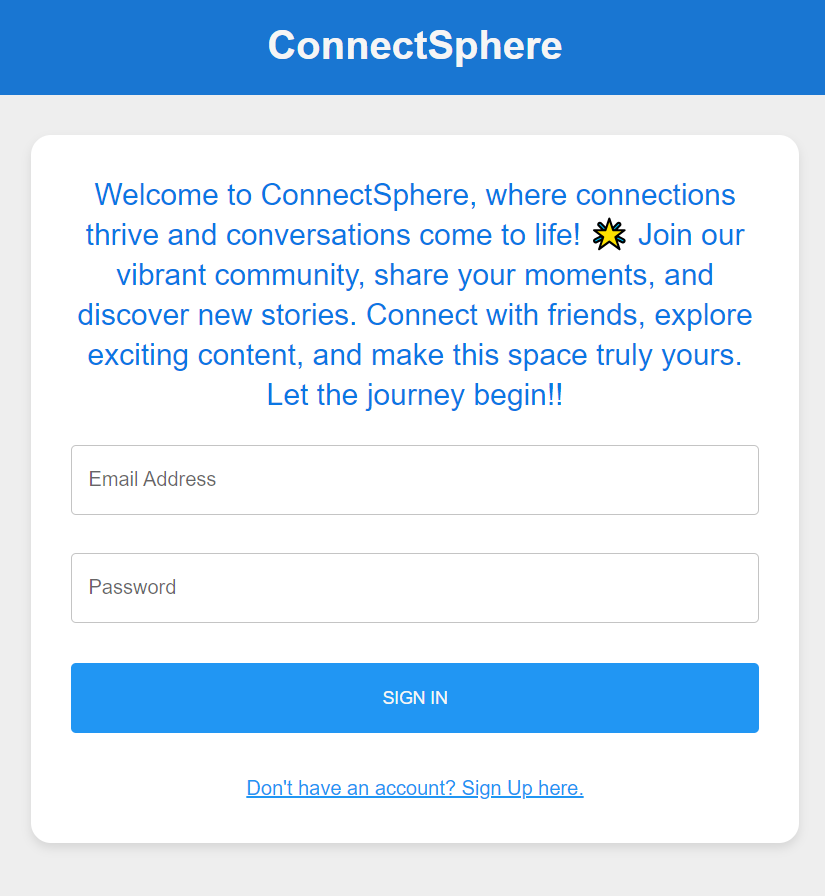
\includegraphics[width=0.7\textwidth]{images/login.PNG}
    \caption{Login Page}
    \label{fig:login}
\end{figure}

\begin{figure}[h!]
    \centering
    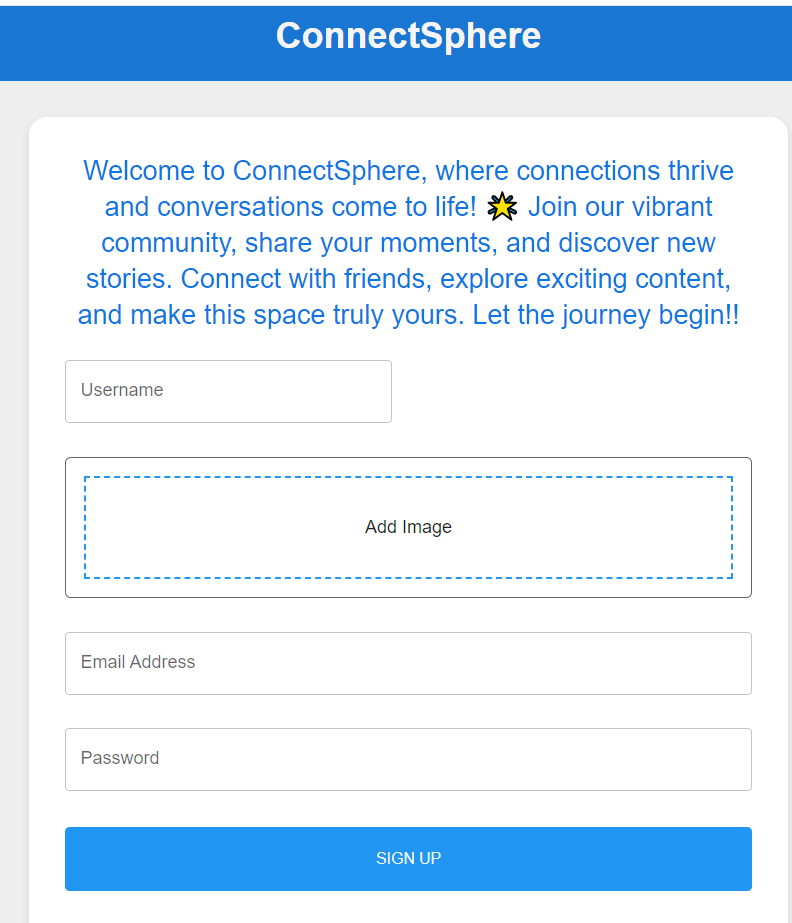
\includegraphics[width=0.7\textwidth]{images/register.PNG}
    \caption{Registration Page}
    \label{fig:register}
\end{figure}

\begin{figure}[h!]
    \centering
    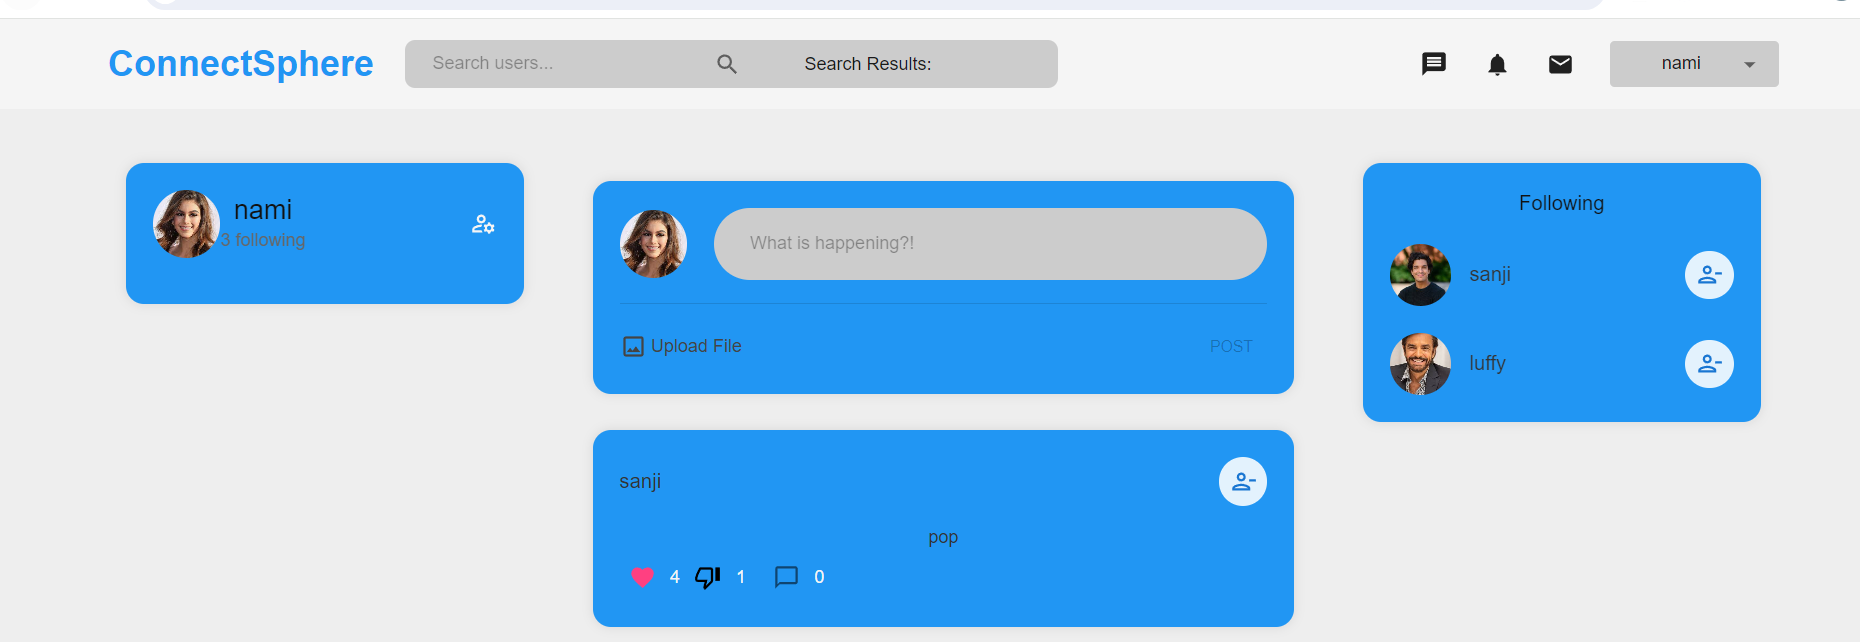
\includegraphics[width=0.7\textwidth]{images/Home.PNG}
    \caption{Home Page}
    \label{fig:home}
\end{figure}

\begin{figure}[h!]
    \centering
    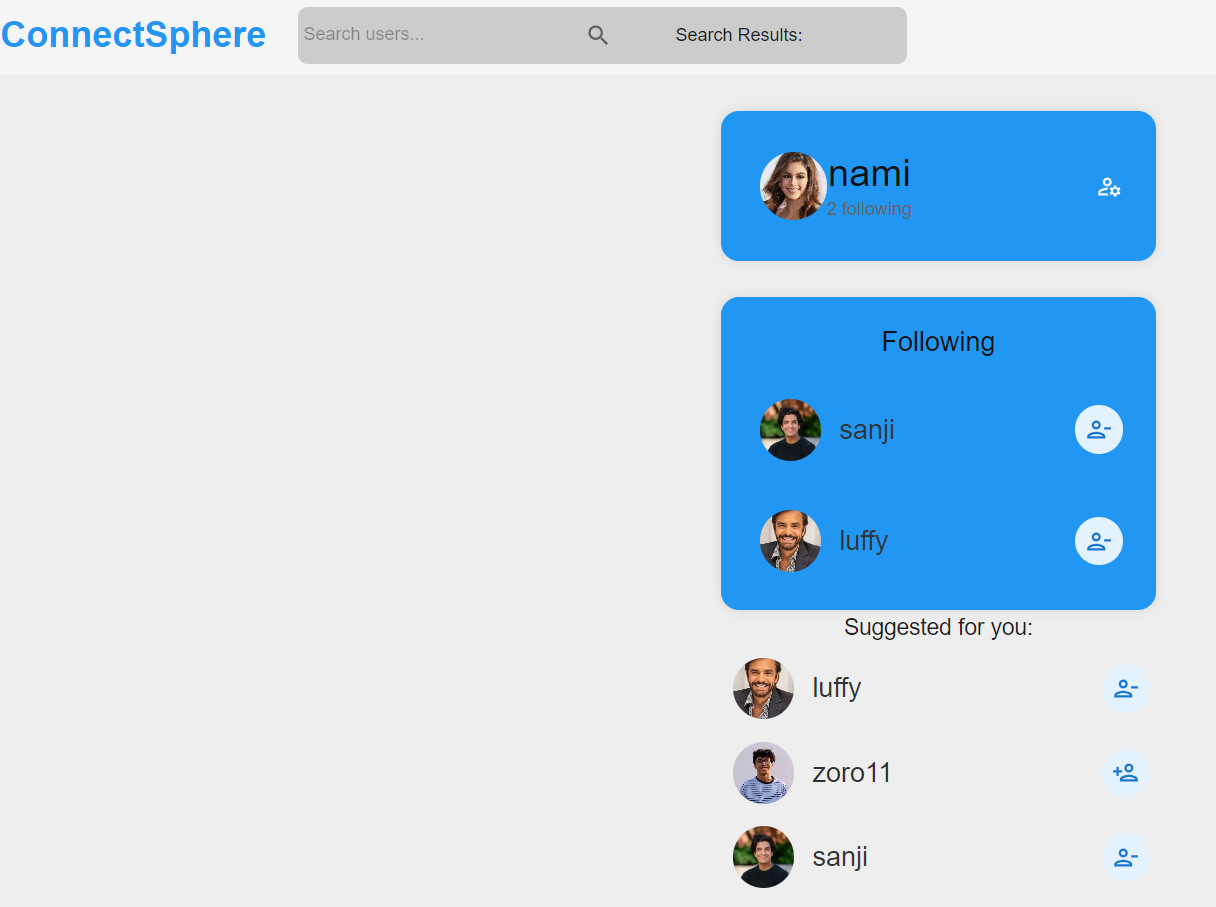
\includegraphics[width=0.7\textwidth]{images/profile.PNG}
    \caption{Profile Page}
    \label{fig:profile}
\end{figure}
\chapter{System Evaluation}
This chapter evaluates the project against the objective set out in the introduction. Results are presented, discussing the system's strengths and weaknesses, and providing key insights into it's overall performance and effectiveness. The process is discussed to evaluate ConnectSphere as a social media platform.

\section{Project Planning}
The project was managed by Jira to help organize tasks and track progress. The project development process was divided into four main phases: project setup, backend development, frontend development, and testing. Each phase had its set of tasks and challenges. The project was set up by defining the project requirements for a social media platform and configuring tools and frameworks. There were some issues like setting up the environment configuration and tools setup but were efficiently resolved. Jira task management features made it possible to implement the project as planned. Backend development focused on implementing the server logic, database integration, and API endpoints. During this phase, tasks related to authentication, data modelling, API design, and file storage were prioritized during this phase. Jira facilitated task management, progress tracking, and issue resolution, ensuring timely completion of backend development tasks. The goal of the frontend development was to create user interfaces, implement client features, and ensure seamless user interaction. The frontend development was more difficult than compared to the backend development because it was more difficult to make it to interact with the backend. Other challenges such as UI design iteration, component integration, and responsive layout. These implementations were managed effectively using Jira's agile boards and task boards. The frontend development took longer to finish because of the challenges. The testing phase included unit testing and integration testing. The testing phase also included a user acceptance test. These tests were conducted to ensure the quality and reliability of ConnectSphere. Jira's issue tracking system helped identify bugs, document test cases, and monitor test progress, enabling application development to provide a stable and robust social media platform. Figure 5.1 depicts the Kanban board, which tracks the progress of five tasks over time.

\begin{figure}[h!]
    \centering
    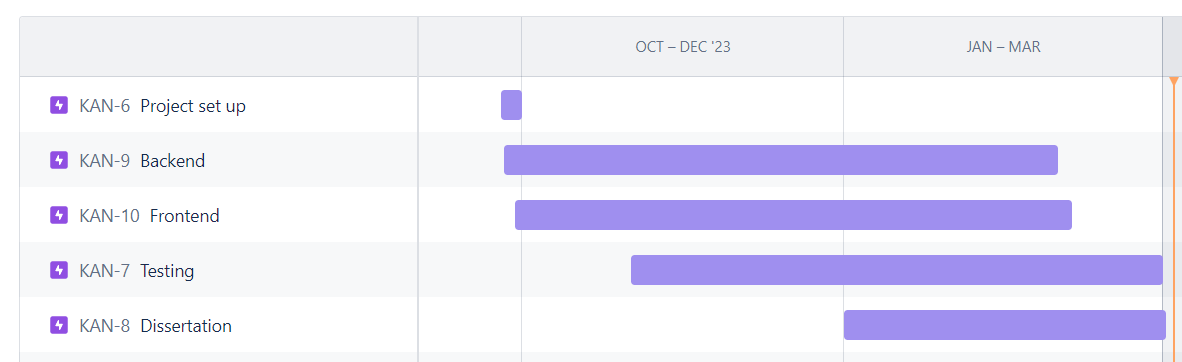
\includegraphics[width=0.7\textwidth]{images/jira.PNG}
    \caption{Jira timeline}
    \label{fig:jira-timeline}
\end{figure}

\section{Objectives Evaluation}
ConnectSphere's overall goal was to be a social media platform that allows users to have an engaging experience with other users and be able to connect in a meaningful way. The project aimed to provide features such as posts, search, chats, messages and comments to enhance user interaction. Creating a secure user authentication to increase application security. These were some of the objectives of the project. The time constraints of the project made it very difficult to develop the application to achieve the objectives. Valuable experiences and skills were gained with the comprehensive development of MERN throughout the entire project. Learned to successfully apply the best practices for MERN stack technologies. The project included the conception, design, and development of a full-fledged web application. This project honed the developer's project management skills and provided valuable experience.


\subsection{Enhance User Engagement}
Implementation of features such as posts, likes, dislikes, videos, images and user interactions have been successfully added. Users can create posts, interact with them through likes and comments, and share images or videos. Dynamic content support for updating and deleting user-generated posts has been successfully implemented, allowing users to manage their content dynamically. This goal was achieved, allowing users to have control over their posts. Users can follow and unfollow other users on ConnectSphere, and a recommendation system has been implemented to suggest users to follow. This goal was achieved by facilitating social connection and enchaining user engagement through recommendation follows. A search has been implemented that allows users to search for another user by username.  Searches are responsive and provide relevant user suggestions. This goal has been successfully achieved, allowing users to efficiently discover and connect with other users. 

User profiles have been created to display key user data and follower counts, providing users with comprehensive user information about their user profiles and social interaction. Successful implementation of key features contribute to the strength of the application. Other features such as a notifications, live chat and messaging have been added to the platform, helping users to stay connected. Time constraints may have impacted the depth of some features or functionality, potentially limiting their scalability. Figure 5.2 depicts the platform's message page.

\begin{figure}[h!]
    \centering
    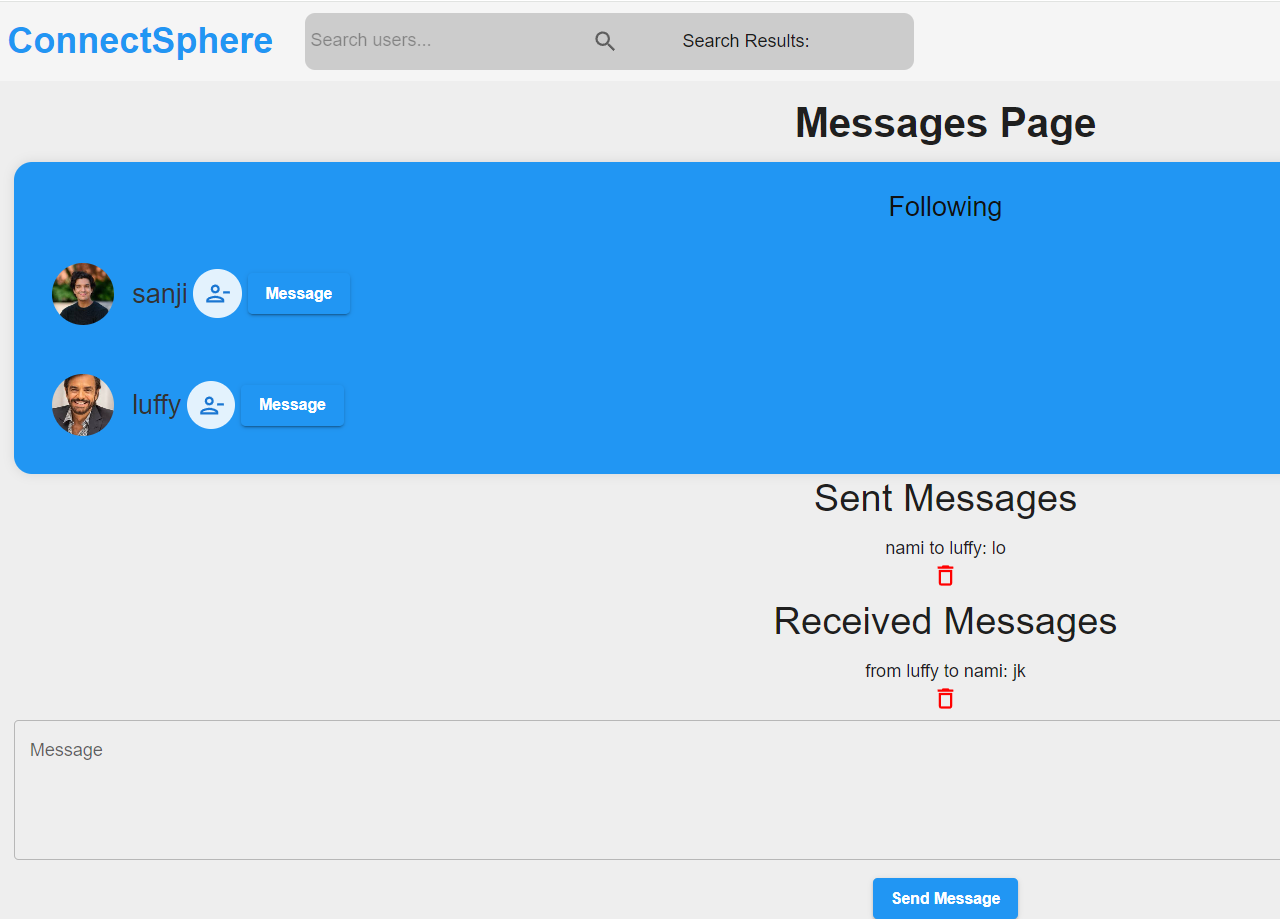
\includegraphics[width=0.7\textwidth]{images/message.PNG}
    \caption{Message Page}
    \label{fig:message-page}
\end{figure}

\subsection{Secure User Authentication}
Secure user authentication is an important part of the application, especially for the sensitive user data or to facilitate interactions between users. In this project, secure authentication was achieved by implementing of token-based authentication. A token-based user authentication system has been implemented for user login and registration. This ensures secure access to accounts and protecting sensitive information. Secure user authentication has been successfully achieved, providing users with a secure and reliable authentication mechanism. User passwords are securely hashed and protected from unauthorized access even in the event of a data breach. Only authenticated users with a valid token can access protected resources using token-based authentication. The web application is resilient against common security vulnerabilities, increasing the overall stability of the authentication system. Using
standard security practices such as JWT for authentication and bcrypt for password hashing ensures user authentication best practices are followed.

Maintaining and updating the authentication system to address evolving security threats and compliance requirements can be complex and resource intensive. The secure user authentication implemented in the project provides a solid foundation for protecting user accounts and sensitive data. Best practices of authentication and continuous system monitoring and updating allow the application to maintain a high level of security and user trust. Although the project includes key features such as authentication, social interaction, and content discovery, it may lack some advanced features found in mature social media platforms. Future iterations of the project may expand functionality. 

\section{Project Testing}
Testing is an essential part of ensuring the reliability and security of ConnectSphere. In this project, Postman was the primary method for testing the backend, covering the multiple scenarios to evaluate the overall performance and functionality of the web application. Other testing methods included unit testing, user acceptance testing, and integration testing. Each API endpoint, including user authentication, post creation, user search and profile management, has been tested by Postman. Various HTTP methods such as GET, PATCH, POST and DELETE were used to communicate with the different endpoints and validate their behavior. Authentication endpoints such as login and registration have been tested to ensure that users can authenticate and securely access protected resources. The design of the API endpoints had to match the expected results. The check included valid inputs, invalid inputs and unauthorized access attempts. Data validation and error handling were part of the process. The input validation and error handling mechanism has been tested to ensure that the application correctly detects and handles invalid input and error conditions. Tests were performed to simulate scenarios such as missing parameters, incorrect queries, and server errors. Some load tests were performed to evaluate the performance of the web application at different levels of concurrent user activity. This was important because scalability issues can arise as the user base grows, requiring optimization to handle increased traffic and load. 

Postman helped identify and resolve bugs, and inconsistencies in the backend API, improving the overall robustness and reliability of the social media platform. Extensive testing of authentication endpoints ensured that user authentication and authorization mechanisms were functioning properly, protecting user accounts and data. All the features such as messaging, login, post creation, search, profile management and interactions have been covered in the testing approach to ensure complete coverage of the application features. Authentication endpoints testing validated the implementation of secure token-based authentication and protected against security vulnerabilities, ensuring compliance with best practices. Integration testing was performed to verify interactions between different components of the web application to ensure seamless functionality across the entire platform. Overall, testing with Postman played a critical role in validating the functionality, security, and performance of the project's backend API.

\section{Database}
Database schemas are designed to efficiently store and retrieve user-related data such as user information, authentication credentials, post, and messages. Collections are organized to support the relationship between users and their posts, followers and other entities, enabling efficient querying and data retrieval. MongoDB enabled fast and efficient queries and provided quick access to user data, posts, and messages. MongoDB scalability and sharding capabilities have provided the foundation for scaling the database as the web application's user base grows. MongoDB flexible schema design allowed for easy adaption to changing application requirements and user needs. integrating MongoDB as the project database provided a solid foundation for storing, managing and retrieving project content. Its flexibility and scalability features met the project requirements and supported the development of a reliable and responsive web application.

\section{Socket.Io}
Socket.Io enabled real-time, two-way communication between the client and server, enabling instant updates and interaction within the application. Users can join chat rooms, send messages, and receive updates without having to manually refresh the entire site. Real-time features like live chats and notifications helps increase user engagement by enabling seamless communication. Users can chat with each other in real time, fostering a sense of communication and enabling meaningful interaction on the platform.
Socket.IO architecture and web sockets support ensures scalable communication with concurrent users. Socket.IO plays a key role in enabling real-time interactions and improving user engagement within the application. Robust features allow users to communicate and stay informed in real time, creating a vibrant user community. A chat room where two users can send messages to each other is shown in Figure 5.3. Figure 5.4 shows the notification page with users liking post notify.

\begin{figure}[h!]
    \centering
    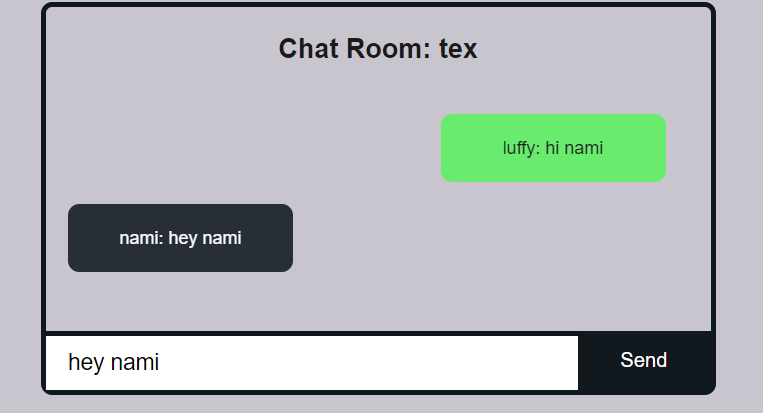
\includegraphics[width=0.7\textwidth]{images/chatroom.PNG}
    \caption{Chat Page}
    \label{fig:chat-rooms}
\end{figure}

\begin{figure}[h!]
    \centering
    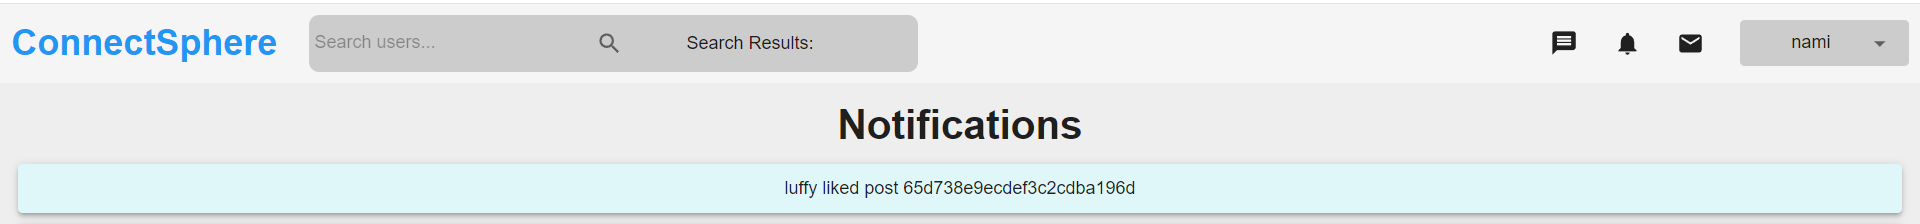
\includegraphics[width=0.7\textwidth]{images/notify.PNG}
    \caption{Notification Page}
    \label{fig:like-notify}
\end{figure}

\section{Frontend and Backend}
\subsection{Frontend}
Frontend components is characterized by its responsiveness and ensuring a seamless experience across different devices. Responsive design principles associated with Material-UI, contribute to a visually appealing and user-friendly interface. State management techniques such as Redux are used effectively to manage application state. Socket.IO integration enables real-time communication and enhance user engagement with features like live chats and notifications. Token-based authentication mechanisms ensure secure user registration and login processes, protect user data and improve overall system security. Authentication follows best practices. The navigation and routing mechanisms created by React Router enables seamless navigation between different views and pages within the web application. Users can easily navigate between features such as user profiles, chat rooms, message inbox page, home page and notification page, improving usability and accessibility. 

Testing strategies such as unit tests and integration tests that help identify code issues and bugs. Frontend development took a long time compared to the backend development. Many HTTP request issues that took some time to solve. Solving these problems took effort to fix.

\subsection{Backend}
The backend is well structured and follows best practices, promoting modularity and scalability. Separation of concerns and use of middleware capabilities contribute to a robust and extensible backend architecture. Token-based authentication mechanisms, implemented using libraries such as JWT, provide secure user authentication and authorization for users. Authentication endpoints comply with MERN standards and include features such as password hashing to improve security. Integration with MongoDB facilitates efficient data storage and retrieval. Data models and schemas are well defined, support CRUD operations, and ensure data consistency and integrity. Integration with Socket.IO enables real time communication between the server and client, facilitating features such as live chats and notifications. The backend worked as expected and was able to perform the task required by the social media platform.  

\subsection{Deployment}
Deploying the web application on Render marks a significant success in the project life-cycle, demonstrating the ability to move from local development to a production environment. Despite the challenges encountered during the deployment process, such as resolving URL issues in frontend HTTP requests. The local-host URLs in the frontend had to be replaced with the new URL provided by Render. For deployment to work, the bcrypt library also had to be removed. Instead, the bcrpty.js library was used to resolve the deployment issues. Deploying the application on Render has several advantages. Render provides scalability allowing ConnectSphere to remain responsive and available during periods of increased activity. Hosting the application on Render improves its reliability and availability. Overall, the successful deployment to Render reflects the ability to overcome challenges and adapt to new environments. This success highlights the project's ability to be used in the real world and creates a solid foundation for development and growth.
\chapter{Conclusion}
In conclusion, this project focused on the development of a social media platform called ConnectSphere. The project's development included enhancing user engagement through the implementation of different features and functions, while ensuring a secure user authentication and dynamic content support. The overall goal was to create a dynamic social media application where users could communicate, share content and connect with others. During the development process, several goals were successfully achieved. Features like posts, likes, dislikes, videos and live chat have improved the user engagement. Token-based methods for login and registrations was used to implement secure user authentication. The application supports dynamic content updates and deletions for user generated posts. The user can follow and unfollow other users on the platform, as well as a recommendation system that helps users in find new contacts. A search function is implemented to allow users to find other users by username, with responsive search results. User profiles are provided to view important details and follow counts. Learning and applying the best practices with technologies like MERN, JWT, Socket.IO and Redux, gaining valuable project building skills. 
\newline \newline
The System Evaluation chapter highlights the strengths and weakness of the system, including the success of secure user authentication, database management with MongoDB and frontend and backend development. Challenges encountered during deployment, such as resolving URL issues for HTTP request, were effectively addressed, leading to a successful deployment to Render. Implementing secure or token-based authentication ensured secure user login and registration, protecting user data and accounts from unauthorized access. JSON web token is the technology is that helps the application apply security to the social media platform. With the token there is a way to know who has access to the application, what their role is and which links have access \cite{haekal2016token}. This add an extra layer of protection and improves the social media platform's strengths.
\newline \newline
During deployment, the system faces challenges including resolving URL issues for HTTP request when transitioning from local development environments to production environment. This deployment issue took multiple attempts to resolve out the problem. The challenges encountered were resolved once the problems were identified. ConnectSphere is successfully deployed to allow users to share content and interact with other users. Scalability is a strong point of the web application. The system has demonstrated scalability in handling a growing user base and content, and offers potential for further expansion and future enhancement. MongoDB is a reliable database that has allowed ConnectSphere to achieve this in a system positive way. MongoDB provides excellent performance and scalability to handle the enormous complexity of web development and usage \cite{aryal2020mern}. Mongoose worked well together with MongoDB because it provided functionality to the features in the database including query building capabilities and business logic in the data \cite{aryal2020mern}. The integration of Socket.IO has enabled the web application to increase user engagement. The features of notifications and live chat features have enabled the social media platform to present dynamic content. The integration with Socket.IO enabled real-time communication and updates to improve the functionality and user experience of the platform.
\newline \newline
While the system generally performed well, there may be areas for performance optimization, particularly when handling a large number of concurrent user interactions or content updates. The platform offers various features for user interaction such as likes, posts, dislikes, and comments, but additional refinements of the user interface and experience could improve usability and engagement. The main aim of the web application is to provide users with an impressive platform to enjoy. While test coverage was performed using tools such as Postman, there may have been areas where test coverage could be expanded to ensure complete validation of the system functionality and performance. There are many error handling inserted into the code to avoid possible problems such as insufficient feedback to users in case of errors. Testing in the frontend development was challenging components had to be carefully integrated to achieve the goal of the web application. 
\newline \newline
React and Material-UI are the two main technologies that played a crucial role in the delivering the frontend application. The user interface has been developed efficiently using React. The component based architecture in React contributed to a responsive and interactive user experience. In order to design the capabilities of the posts to obtain dynamic support, various components have been developed. Material-UI was used to develop the user interface components, providing a rich set of customizable user interface elements that bring consistency and aesthetic appeal to the web application. The fresh design make the social media platform look creative and intuitive. Material-UI has significantly improved the user experience in ConnectSphere. Other frontend technologies such as Redux, Formik and Yup, React Router and Dropzone also played an important role in the creation of ConnectSphere. Redux efficiently handles state management and works with local storage. Formik and Yup handled the form validation of login and registration. Dropzone allows you to upload image and video. React Router was responsible for navigation in the web application. Node.js and Express.Js are the two main technologies responsible for the backend of the project. The development of API, middleware and request paths has been simplified through the use of Node.js and Express. MongoDB is where the data for the code is stored, accommodating the dynamic content requirements of the web application. Overall, the project demonstrated the ability to create a functional and engaging social media platform while overcoming various technical challenges. There is potential for additional refinements and improvements in the future to expand the capabilities of the platform and improve the user experience.
\appendix
\chapter{GitHub repository link}

\section{Applied Project and Minor dissertation}

The URL below directs to the project's GitHub repository. The complete source code, README, dissertation report, screen-cast link and other resources are available here.

\href{https://github.com/davidamankwah/Final_YearProject}{https://github.com/davidamankwah/Final\textunderscore YearProject}




%------------------------------------------------------------------------------------------------------	
% Generate the bibliography. You may have to build the document more than once before all of the
% references and processed and cited correctly.
% WARNING: Don't mess with any of the following unless you know what you are doing.
%------------------------------------------------------------------------------------------------------	
\bibliographystyle{unsrt}
\bibliography{references.bib}
\end{document}